\documentclass[runningheads,twocolumn,envcountsame,envcountsect]{llncs}
\usepackage{fontspec}
\setmainfont{texgyretermes}[Extension=.otf,UprightFont=*-regular,BoldFont=*-bold,ItalicFont=*-italic,BoldItalicFont=*-bolditalic]
\setsansfont{texgyreheros}[Extension=.otf,UprightFont=*-regular,BoldFont=*-bold,ItalicFont=*-italic,BoldItalicFont=*-bolditalic]
\usepackage{amsmath,amssymb,booktabs,tabularx,array,graphicx}
\usepackage{marvosym}
\usepackage{enumitem,xcolor,tikz,microtype,xurl}
\usepackage{hk261_compact}
\usepackage[hidelinks]{hyperref}
\usetikzlibrary{arrows.meta,positioning,fit,backgrounds,calc}
\definecolor{ink}{gray}{0}
\definecolor{teal}{gray}{.18}
\definecolor{blue}{gray}{.28}
\newcolumntype{P}[1]{>{\raggedright\arraybackslash}p{#1}}
\newcolumntype{Y}{>{\raggedright\arraybackslash}X}
\newcolumntype{C}{>{\centering\arraybackslash}X}
\newcommand{\E}{\mathbb E}
\newcommand{\TV}{\operatorname{TV}}
\newcommand{\Var}{\operatorname{Var}}
\newcommand{\Cov}{\operatorname{Cov}}
\newcommand{\BQ}{GeoI-BQ}
\hypersetup{pdftitle={GeoI-BQ: Giới hạn tiết lộ toàn bộ transcript cho truy vấn vị trí trên mạng đường},
pdfauthor={Hanh Ngo-Minh; Phan Trong Nhan},
pdfsubject={Bản tiếng Việt để tác giả đọc và chỉnh sửa}}
\title{GeoI-BQ: Giới hạn tiết lộ toàn bộ transcript\\
cho truy vấn vị trí trên mạng đường}
\titlerunning{GeoI-BQ: Bảo vệ transcript truy vấn vị trí}
\author{Hanh Ngo-Minh\inst{1,2}\textsuperscript{\Letter} \and
Phan Trong Nhan\inst{1,2}}
\authorrunning{Hanh Ngo-Minh and Phan Trong Nhan}
\institute{Faculty of Computer Science and Engineering, Ho Chi Minh City University of
Technology (HCMUT),\\
268 Ly Thuong Kiet, District 10, Ho Chi Minh City, Vietnam.
\and
Vietnam National University Ho Chi Minh City (VNU-HCM),\\
Linh Trung Ward,
Thu Duc District, Ho Chi Minh City, Vietnam.\\
\email{\{nmhanh.sdh241, nhanpt\}@hcmut.edu.vn}\\
\Letter\ Tác giả liên hệ: \email{nmhanh.sdh241@hcmut.edu.vn}}
\newcommand{\paperabstract}{%
\begin{abstract}
Chuỗi truy vấn vị trí tạo thành một transcript (toàn bộ thông tin trao đổi),
mà mức bảo vệ không thể được suy ra chỉ từ từng điểm nhiễu riêng lẻ.
Chúng tôi đề xuất GeoI-BQ, kết hợp điểm tham chiếu trên mạng đường thỏa
geo-indistinguishability, phép kiểm tra tái sử dụng có bảo vệ và cơ chế lấy mẫu
chung một đoạn truy vấn với mức tiết lộ bị chặn. Lịch phân bổ ngân sách có tổng
hữu hạn giới hạn tiết lộ của transcript mà không cần biết trước thời lượng
chuyến đi. Với các giả thiết rõ ràng về miền hỗ trợ, thời gian, trạng thái và
nhà cung cấp, chúng tôi suy ra cận tỷ số xác suất đầu ra cho toàn hệ thống và
cận suy luận vị trí phụ thuộc prior. Phân tích utility tách mức tăng điểm lập
kế hoạch khỏi chất lượng dịch vụ thật, đồng thời chặn độ lệch so với một cơ chế
công khai tương ứng. Thực nghiệm có kiểm soát trên dữ liệu mô phỏng so sánh ba
bản điều chỉnh từ paper và hai đối chứng, với 20 nhóm tuyến TEST và 120 lượt
chuyến đi--lấy mẫu. GeoI-BQ đạt Recall@5 toàn phiên 99.595\% và Hit100
0--0.188\% trên năm tác vụ định vị, sử dụng 155 truy vấn tọa độ trong phiên
600 giây. Cơ chế nền không thích nghi có Recall nhỉnh hơn; việc thiết bị đã
có toàn bộ dữ liệu tham chiếu tĩnh cũng giới hạn lập luận về sự cần thiết của
truy vấn online. Kết quả hỗ trợ một cơ chế bảo vệ transcript có điều kiện và
phân tích đánh đổi tái lập được, chưa phải chứng nhận triển khai hay tái lập
chính thức các paper gốc.

\keywords{Riêng tư quỹ đạo \and Geo-indistinguishability \and
Dịch vụ vị trí \and Hợp thành thích nghi \and Truy hồi địa điểm}
\end{abstract}}
\AtBeginDocument{%
\renewcommand{\abstractname}{Tóm tắt.}%
\renewcommand{\keywordname}{Từ khóa:}%
\renewcommand{\figurename}{Hình}%
\renewcommand{\tablename}{Bảng}%
\renewcommand{\refname}{Tài liệu tham khảo}%
\renewcommand{\ackname}{Lời cảm ơn.}%
\renewcommand{\propositionname}{Mệnh đề}%
\renewcommand{\theoremname}{Định lý}%
}
\begin{document}
\maketitle
\section{Giới thiệu}\label{sec:intro}
Dịch vụ bản đồ giúp tìm đường và địa điểm trong lúc di chuyển. Nếu nhiều chuyến thường kết thúc gần một bệnh viện, bên quan sát có thể phỏng đoán về sức khỏe hoặc thói quen dù người dùng chỉ tới thăm người thân. Tính đặc trưng của dấu vết di chuyển làm rủi ro này đáng quan tâm~\cite{mobilityunique}.

Câu hỏi chúng tôi đặt ra là sau cả chuyến đi, chuỗi trao đổi ấy giúp nhà
cung cấp phân biệt hai quỹ đạo thật đến mức nào? Geo-indistinguishability
(Geo-I) cho ta điểm xuất phát bằng cách giới hạn tỷ số xác suất quan sát cùng
một đầu ra tại hai vị trí thật~\cite{geoi}. Để mở rộng lập luận ra cả phiên,
ta phải tính cả những lần thiết bị đọc lại GPS để quyết định giữ hay đổi điểm
tham chiếu. Chi phí của quan sát mới cũng là cơ sở của các cơ chế bảo vệ dùng
dự đoán~\cite{predictive}.

Về phía người dùng, điều quan trọng là danh sách địa điểm (POI) nào thực sự
hiện trên màn hình. Truy vấn từ nhiều vị trí có thể thu về đủ địa điểm để
điện thoại xếp hạng theo nhu cầu thật~\cite{ev}. Vì vậy, chúng tôi so danh sách
người dùng nhận được với đáp án cho cùng yêu cầu tại GPS thật trên toàn bộ
danh mục. Cách đo này áp dụng được khi đầu ra công khai là một tọa độ, một
tập điểm thật và giả, hoặc một chuỗi có thêm truy vấn giả. Các công trình về
phát hành quỹ đạo ngoại tuyến có mục tiêu sử dụng khác~\cite{transprotect,semantic,fake,sok}.

Chúng tôi xác định mười kịch bản theo thông tin bên quan sát muốn suy ra
và phần chuỗi trao đổi (transcript) họ được thấy.

\smallskip\noindent\textbf{Vị trí và đường đã đi.}
Từ một gói, bên quan sát ước lượng GPS hiện tại (S1). Với chuỗi dài hơn,
họ có thể tìm nơi dừng (S2) hoặc khôi phục vị trí ở từng mốc thời gian (S3).
Ở S2, dữ liệu chỉ cho phép dùng tọa độ trung bình trong phút cuối làm đại
diện cho nơi dừng. Khi cho xem toàn phiên, ta còn đo được khả năng suy ra
điểm xuất phát (S9) và điểm kết thúc (S10). Đây là năm tác vụ định vị chính.

\smallskip\noindent\textbf{Liên kết và dự đoán.}
Hai phiên có thuộc về cùng một người hay phương tiện (S4)? Dữ liệu chỉ có
nhãn nhóm tuyến, nên phép thử là xác định hai phiên có cùng nhóm hay không.
Với suy luận tương lai, chúng tôi xét hai quyết định khác nhau trên mạng
đường. S5 dự đoán nhánh kế tiếp trong hai nhánh khả dĩ. S6 chọn một trong
hai đích đến khi đã thấy người dùng rẽ.

\smallskip\noindent\textbf{Nội dung và người đi cùng.}
Ở S7, ta giữ nguyên chuyến đi rồi đổi yêu cầu trên thiết bị để kiểm tra xem
nội dung yêu cầu có làm thay đổi transcript hay không. S8 xét một nguồn
thông tin khác mà nhà cung cấp có thể có. Khi căn hai luồng truy vấn theo
thời gian, quan sát thêm người đi cùng giúp định vị người dùng đến mức nào?


GeoI-BQ giữ điểm tham chiếu đã bảo vệ trên mạng đường. Từ lịch sử các điểm
tham chiếu, thiết bị ước lượng một phân phối vị trí (belief) để chọn cả đoạn
truy vấn kế tiếp. Nghiên cứu có ba đóng góp.
\begin{itemize}
\item Một khung mô tả từng kịch bản theo mục tiêu suy luận, lịch sử được quan sát và dữ liệu tham chiếu để chấm.
\item Một cơ chế truy vấn theo đoạn dựa trên Geo-I, với cận tiết lộ cả phiên và điều kiện bảo đảm chất lượng dịch vụ.
\item Đối chiếu sáu phương án trên cùng tác vụ, có khoảng tin cậy, chi phí và các thước đo gốc áp dụng được.
\end{itemize}
Trong thử nghiệm, thiết bị đã có toàn bộ danh mục tĩnh và phương án nền
công khai đạt Recall nhỉnh hơn cơ chế thích nghi. Hai điều kiện này ảnh hưởng
đến cách diễn giải lợi ích của truy vấn trực tuyến.
Các phần~\ref{sec:related}--\ref{sec:conclusion} trình bày nghiên cứu liên quan,
phương pháp và chứng minh, kết quả thực nghiệm và kết luận.

\section{Nghiên cứu liên quan}\label{sec:related}
Geo-I, dự đoán, hợp thành và hậu xử lý cung cấp cơ sở
lý thuyết~\cite{geoi,predictive,dworkroth}. EV querying kết hợp Geo-I xấp xỉ,
điểm giả và lựa chọn local~\cite{ev}; PTPPM xét bảo vệ cá nhân hóa trên mạng
đường dưới tương quan~\cite{ptppm}. Tóm tắt chương trình IWPE 2026 cũng đề cập
thích nghi theo đường và dự đoán di chuyển~\cite{iwpe26}; chúng tôi không suy
diễn một đặc tả đầy đủ khi chỉ có bản tóm tắt.

TransProtect sinh tọa độ thay thế theo ngữ cảnh~\cite{transprotect}.
Semantic correlation tạo tập điểm thật và giả~\cite{semantic}, còn fake-query
insertion chèn thêm các sự kiện chỉ chứa truy vấn giả~\cite{fake}.
Mỗi dạng đầu ra dẫn tới cách đo suy luận và dịch vụ khác nhau. Các bản triển
khai trong nghiên cứu này lần lượt thay thế bằng bộ dự đoán Markov, ngữ nghĩa
OSM/thực nghiệm và dự đoán dựa trên đường/lịch sử. Đây là các bản điều chỉnh
đã được rà soát, không phải bản tái lập chính thức.

CPCROK giải quyết khả năng liên kết bí danh/beacon của phương
tiện~\cite{cpcrok}; DP-FETC xét phát hành quỹ đạo offline~\cite{dpfetc}.
Hai bài toán không ánh xạ trực tiếp sang truy hồi POI online. SoK về sinh
quỹ đạo cũng nhấn mạnh đơn vị bảo vệ và giả thiết đánh giá~\cite{sok}.
Bảng~\ref{tab:related} giữ cửa sổ khảo sát đã rà soát
(28/10/2023--28/10/2026); các nền tảng cũ được dẫn riêng.
Đóng góp được xem xét ở đây là kênh công bố có cận tiết lộ cùng phân tích
liên kết của nó, không phải nguyên lý Geo-I mới hay một metric dùng cho mọi bài toán.
\begin{table*}[t]\centering\footnotesize
\caption{Nghiên cứu gần đây: dạng đầu ra, phạm vi tác vụ và tình trạng bằng chứng.}\label{tab:related}
\begin{tabularx}{\linewidth}{@{}P{2.5cm}P{2.05cm}P{2.15cm}YP{2.35cm}@{}}\toprule
\textbf{Công trình} & \textbf{Đầu ra} & \textbf{Phạm vi} & \textbf{Metrics privacy / utility} & \textbf{Trong nghiên cứu này} \\
\midrule
TransProtect (2024)\cite{transprotect} & Tọa độ tổng hợp & D: S1, S3; P: S2 & EIE / VehiTrack; sai lệch chi phí di chuyển & Điều chỉnh Markov \\
Semantic (2026)\cite{semantic} & Tập điểm thật + giả & D: S1; P: S2, S3 & ASR; DER; thời gian sinh & Điều chỉnh OSM/thực nghiệm \\
Fake queries (2026)\cite{fake} & Tập hỗn hợp và chỉ giả & D: S1, S3; P: S2 & ASR; số đường không phân biệt được; thời gian/RSS & Điều chỉnh đường/lịch sử \\
EV querying (2024)\cite{ev} & Truy vấn nhiễu/giả & P: S1--S3 & Geo-I xấp xỉ; IBU/Wasserstein; chi phí riêng tư & Chỉ khảo sát; tương tác Edge khác \\
CPCROK (2025)\cite{cpcrok} & Bí danh / beacon & P: S4 & Liên kết lại; tuyến giả; truyền thông & Tương tác VANET khác \\
DP-FETC (2025)\cite{dpfetc} & Quỹ đạo offline & P: S3, S8--S10 & DP; thông tin tương hỗ; JSD & Dạng phát hành khác \\
PTPPM (2025)\cite{ptppm} & Nhiễu trên đường & U: S1, S3 & Geo-I; sai lệch / QoS & Preprint; chưa có đối chứng đã rà soát \\
SoK (2024)\cite{sok} & Khảo sát tổng hợp & Không là đối chứng & Đơn vị bảo vệ; tái dựng; utility & Ngữ cảnh và hướng dẫn đánh giá \\
\bottomrule\end{tabularx}
\par\smallskip\raggedright D: đánh giá trực tiếp tác vụ trong giả thiết của paper; P: giao nhau một phần; U: chưa đủ bằng chứng đã rà soát để kết luận mạnh hơn. Chưa xác lập bảo vệ trực tiếp cho scenario không được liệt kê. D không có nghĩa bảo vệ trước mọi attacker.
\end{table*}


\section{Phương pháp đề xuất}\label{sec:method}
\subsection{Khung hệ thống}\label{sec:system}
Gọi $V$ là miền trạng thái hữu hạn của mạng đường có hướng, với tọa độ chiếu
$a_v$. Khoảng cách Euclid dùng cho privacy/định vị; chi phí có hướng dùng để
kiểm tra đường đi và xếp hạng dịch vụ. GPS $x_t$ và nhu cầu $\psi_t$ chỉ ở local.
Nhà cung cấp biết thuật toán và ngữ cảnh công khai $C$, đồng thời quan sát
tọa độ Q theo thứ tự, đồng hồ, truy vấn chung, phản hồi và lần thử lại.
Họ không thấy điểm tham chiếu $Z$, belief, sổ ngân sách hay kết quả đã xếp hạng
(Hình~\ref{fig:system}).

\begin{figure}[!ht]\centering
\resizebox{\columnwidth}{!}{\begin{tikzpicture}[>=Latex,
 box/.style={draw=ink!65,rounded corners=2pt,fill=white,text width=3.9cm,
 align=center,inner sep=5pt,font=\small},
 arr/.style={->,thick,draw=ink}]
\node[box,draw=teal,fill=teal!4] (model) at (0,0)
{\textbf{Thiết bị: GeoI-BQ}\\GPS riêng $\to Z$/belief $\to$ Q};
\node[box] (local) at (0,-1.7)
{\textbf{Xử lý đáp án tại local}\\Cache; lọc/sắp xếp bằng GPS và $\psi$};
\node[box,text width=2.5cm] (server) at (5.5,-.7)
{\textbf{LBS / bên quan sát}\\Thấy Q, đồng hồ,\\truy vấn và phản hồi};
\node[box,text width=3.9cm] (context) at (0,1.45)
{\textbf{Ngữ cảnh thiết kế công khai}\\Đường và toàn bộ tham chiếu thử nghiệm};
\node[box] (out) at (0,-3.1)
{\textbf{Đầu ra cho người dùng}\\Toàn danh sách phù hợp đã sắp xếp};
\draw[arr] (context)--(model);
\draw[arr] (model.east)--node[above,font=\scriptsize,align=center]{truy vấn\\chung}(server.north west);
\draw[arr,blue] (server.south west)--node[below,font=\scriptsize]{POI}(local.east);
\draw[arr] (local)--(out);
\draw[arr,teal] (model.west)--++(-.4,0)|-(local.west);
\begin{scope}[on background layer]
\node[fit=(model)(local)(context)(out),draw=teal,fill=teal!2,rounded corners,inner sep=8pt] {};
\end{scope}
\end{tikzpicture}
}
\caption{Ranh giới giữa thiết bị tin cậy và nhà cung cấp. Prototype đã nạp toàn
bộ dữ liệu tham chiếu tĩnh mà nhà cung cấp thử nghiệm sử dụng.}\label{fig:system}
\end{figure}

Bảo đảm đòi hỏi miền hỗ trợ ứng viên chung và trọng số nền công khai dương
tại mỗi tiền tố hành động mở rộng, kể cả trạng thái làn của điểm giả; kernel
không gian lý tưởng; bit ngẫu nhiên Q mới, đều và độc lập; trạng thái phiên
đã cam kết, không thể quay lui và khôi phục đầy đủ các thành phần trước Q;
ranh giới phiên/đồng hồ công khai; cùng quy luật phản hồi có điều kiện của
nhà cung cấp khi truy vấn/lịch sử giống nhau. Di chuyển được coi là ngoại sinh.
Tài khoản/IP, thời điểm bắt đầu/kết thúc riêng tư và phản hồi tác động tới
di chuyển là các kênh cần xét thêm. Kết quả cache đòi hỏi metadata hợp lệ và
thứ tự xếp hạng chung. Số học nguyên ở bước Q tự nó chưa chứng nhận toàn bộ
triển khai có số thực dấu phẩy động~\cite{mironov}.

Bộ khởi tạo prototype có đầy đủ dữ liệu tham chiếu/phản hồi khớp nhà cung cấp
tĩnh. Mặt nạ POI đã nhận giới hạn câu trả lời được đo, nhưng chưa tạo cách ly
thông tin: client offline có cùng dữ liệu có thể trả lời chính xác mọi yêu
cầu tĩnh đã định nghĩa. Chi phí thu thập và cập nhật dữ liệu là vấn đề riêng.

\subsection{Luồng xử lý}
\subsubsection{Điểm tham chiếu và belief đã bảo vệ.}
Cơ chế hàm mũ trên đường (REM) lấy mẫu trực tiếp một trạng thái đường:
\begin{equation}
R_u(v\mid x)=
\frac{e^{-u\|x-a_v\|/2}}{\sum_{w\in V}e^{-u\|x-a_w\|/2}},
\quad Z=a_v. \label{eq:rem}
\end{equation}
Ở lần đọc GPS tiếp theo được phép, tham chiếu cũ $h$ được kiểm tra bằng
\begin{equation}
D_t=\mathbf1\{\|x_t-h\|+\xi_t>\theta\},
\quad \xi_t\sim\operatorname{Lap}(0,1/u). \label{eq:test}
\end{equation}
Tái sử dụng tốn $u$; kiểm tra rồi tạo mới tốn $2u$; REM ban đầu tốn $u$.
Bộ lọc ngân sách dự phòng chi phí tối đa của bước kế tiếp trước khi đọc GPS:
\begin{equation}
u\sum_i c_i\le Mu\le C_s,\qquad
M=\lfloor C_s/u\rfloor,\quad c_i\in\{0,1,2\}. \label{eq:cap}
\end{equation}
Cấu hình đã đóng băng dùng $u=B/(2H_{\rm cfg})$,
$B=0.24\,\mathrm m^{-1}$ và $H_{\rm cfg}=12$, suy ra $u=0.01\,\mathrm m^{-1}$,
$M=23$, $C_s=0.23\,\mathrm m^{-1}$ và $\theta=200$ m.
Tổng quát, $C_s\le\log(R_\star)/d_\star$ đủ để chặn tỷ số không gian bởi
$R_\star$ khi $D_\infty\le d_\star$. Hết ngân sách sẽ ngừng đọc GPS cho cơ chế
bảo vệ, nhưng không ngừng gửi truy vấn.

Belief trên các trạng thái đại diện dự đoán bằng mô hình di chuyển công khai
và chỉ cập nhật khi thực sự có quan sát đã bảo vệ:
\begin{align}
b_t^-(s)&=\sum_r b_{t-1}(r)T_{\Delta t}(r,s),\\
b_t(s)&\propto b_t^-(s)\ell_t(Z_t\mid s,h). \label{eq:belief}
\end{align}
Hàm phát xạ kết hợp khối xác suất tại tham chiếu được tái sử dụng với xác suất
REM khi tạo mới. Bỏ qua lần đọc thì chỉ dự đoán; Z lặp lại không phải phép
đo độc lập. Belief xấp xỉ này chưa được chứng nhận hiệu chuẩn trên người dùng thật.

\subsubsection{Chọn đoạn truy vấn và trả lời local.}
Mỗi hành động gồm ba khung K5 (mỗi khung năm điểm Q), nối nhau bằng chuyển
động khả thi trên đường có hướng. Ngữ cảnh công khai cùng hành động/phản hồi
giả trước đó xác định thư viện và trọng số; GPS, Z, belief và request không
được dùng để loại ứng viên khỏi miền hỗ trợ. Đứng yên cung cấp lựa chọn khả
thi chung; nếu xây dựng thư viện công khai rỗng thì ghi nhận là thất bại.
Bộ lập kế hoạch đã đóng băng dùng độ rộng 24, trọng số mới lạ/tầm xa bằng bốn
và thang di chuyển 60 s. Tài liệu bổ sung đặc tả trọng số cùng điểm đại diện
$g_a(s)$ bị chặn, dựa trên độ phủ cache và độ gần.

Điểm $v_a=\sum_sb(s)g_a(s)$ được chuẩn hóa/lượng tử thành $z_a\in[0,1]$
với độ phân giải 65536. Tại đoạn $j$,
\begin{align}
\varepsilon_{Q,j}&=\frac{\Gamma_Q}{j(j+1)},&
\alpha_j&=\frac{\widehat\varepsilon_{Q,j}}{2+\widehat\varepsilon_{Q,j}},\\
\mu_j&=\sum_aw_az_a,&
p_a&=w_a[1+\alpha_j(z_a-\mu_j)]. \label{eq:kernel}
\end{align}
Ở đây $\widehat\varepsilon_{Q,j}\le\varepsilon_{Q,j}$ là hạn mức hữu tỷ làm
tròn xuống; thực nghiệm dùng $\Gamma_Q=1$. Trọng số tích lũy nguyên chính xác
thực hiện phân phối này với điều kiện các bit đầu vào đều.

Đoạn đã cam kết phát các khung tại 0, 20 và 40 s; đoạn tiếp theo bắt đầu ở
60 s (Hình~\ref{fig:model}). Các lần đọc GPS cho cơ chế bảo vệ cách nhau ít
nhất 60 s; GPS local hiện tại vẫn có thể dùng xếp hạng ở mỗi nhịp dịch vụ.
Mỗi Q yêu cầu cùng sáu loại POI, $L60$ cho mỗi loại. Thiết bị loại trùng/lưu
cache, sau đó lọc và sắp xếp riêng theo $\psi_t$. Người dùng nhận toàn bộ danh
sách phù hợp; top năm chỉ là tập tham chiếu khi đánh giá.

\begin{figure*}[t]\centering
\resizebox{.94\textwidth}{!}{\begin{tikzpicture}[>=Latex,
 box/.style={draw=ink!65,rounded corners=2pt,fill=white,text width=4cm,
 align=center,inner sep=6pt,font=\small},
 side/.style={draw=blue!60,fill=blue!4,rounded corners=2pt,text width=4cm,
 align=center,inner sep=5pt,font=\small},
 arr/.style={->,thick,draw=ink}]
\node[box] (rem) at (0,0)
{\textbf{1. Lịch sử không gian đã bảo vệ}\\Đọc GPS khi được phép: REM $Z$\\Kiểm tra giữ/đổi riêng tư; giới hạn $C_s$};
\node[box] (belief) at (5.6,0)
{\textbf{2. Belief từ dữ liệu đã bảo vệ}\\Dự đoán chuyển động +\\cập nhật theo quan sát đã bảo vệ};
\node[box,draw=teal] (choose) at (11.2,0)
{\textbf{3. Chọn chung cả đoạn Q}\\Thư viện/nền chung; hiệu chỉnh có cận\\Lưu bền bộ đếm $j$ và hành động};
\node[box] (send) at (11.2,-2.1)
{\textbf{4. Cam kết và công bố}\\K5 tại 0/20/40 s; đoạn mới tại 60 s\\Truy vấn sáu loại chung, L60};
\node[box] (local) at (5.6,-2.1)
{\textbf{5. Xử lý dịch vụ tại local}\\Hợp/cache các POI hợp lệ\\Lọc/sắp xếp bằng GPS hiện tại + $\psi$};
\node[side] (input) at (0,1.7)
{\textbf{Luồng GPS riêng tư}};
\node[side,text width=6.9cm] (public) at (8.4,1.7)
{\textbf{Ngữ cảnh công khai:} đường, proxy, đồng hồ, Q/phản hồi trước};
\node[side] (output) at (0,-2.1)
{\textbf{Đầu ra}\\Toàn danh sách phù hợp đã sắp xếp};
\node[side] (provider) at (11.2,-3.8)
{\textbf{LBS bên ngoài:} Q $\to$ POI};
\draw[arr] (input)--(rem);
\draw[arr] (rem)--(belief);
\draw[arr] (belief)--(choose);
\draw[arr] (choose)--(send);
\draw[arr] (local)--(output);
\draw[arr,blue] (send)--(provider);
\draw[arr,blue] (provider.west)-|node[below,pos=.3,font=\scriptsize]{phản hồi POI}(local.south);
\draw[arr,dashed,blue] (public.south west)--(belief.north);
\draw[arr,dashed,blue] (public.south east)--(choose.north);
\draw[arr,dashed] (local.north)--(5.6,-1.05)-|(choose.west);
\node[font=\scriptsize,fill=white,inner sep=2pt] at (7.3,-1.05) {chỉ cache công khai};
\begin{scope}[on background layer]
\node[fit=(rem)(belief)(choose)(send)(local),draw=teal,fill=teal!2,
 rounded corners,inner sep=10pt] (boundary) {};
\end{scope}
\node[font=\scriptsize\bfseries,text=teal,anchor=north west,fill=white,inner sep=2pt]
at (boundary.north west) {GEOI-BQ TRÊN THIẾT BỊ};
\end{tikzpicture}
}
\caption{Luồng GeoI-BQ. Lịch sử không gian đã bảo vệ chấm điểm cho thư viện
đoạn công khai chung; các khung đã cam kết truy hồi POI để xếp hạng local.
Chỉ thông tin cache công khai được dùng lại khi tạo ứng viên.}\label{fig:model}
\end{figure*}

Hình~\ref{fig:walkthrough} theo dõi một chuyến TEST đã lưu, được chọn vì
đường đi có nhiều lần rẽ. Tại 20/40 s, belief chỉ dự đoán, không đọc GPS cho
cơ chế bảo vệ; kiểm tra rồi tạo mới tại 60/120/180 s đều tốn hai đơn vị.

\begin{figure*}[t]\centering
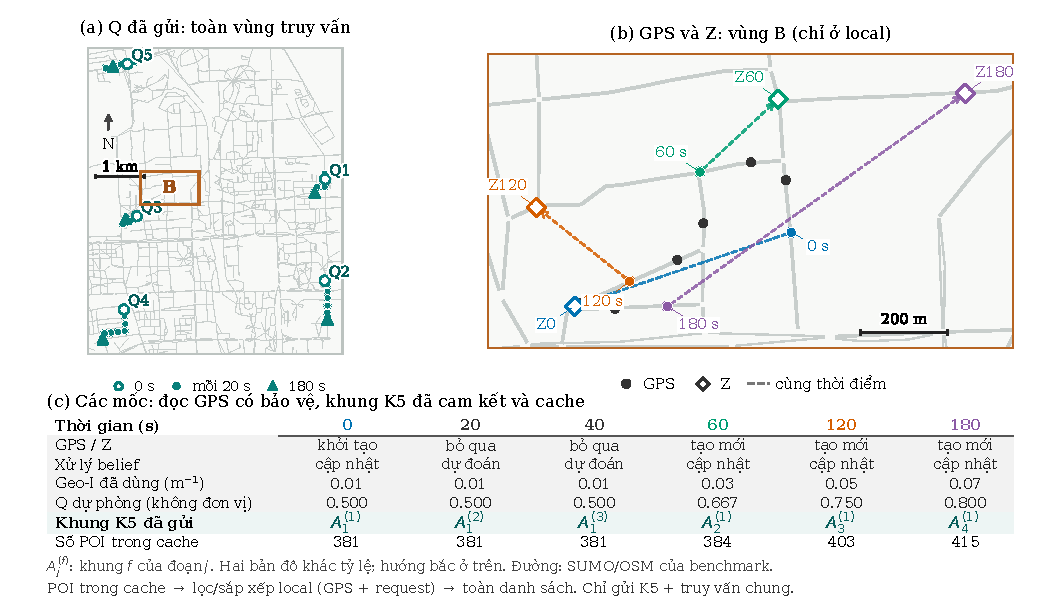
\includegraphics[width=\textwidth]{figure_walkthrough.pdf}
\caption{Chuyến đã lưu \texttt{cache-046\_day7}, 0--180 s.
(a) Cả năm luồng Q; khung B định vị phần phóng lớn riêng ở (b).
GPS tô đặc và Z rỗng có nhãn/màu theo cùng thời điểm; nét đứt thể hiện độ
lệch tham chiếu, không phải đường di chuyển.
(c) Một số mốc và khung đã cam kết; ba khung đầu thuộc cùng đoạn.
Z, belief, sổ ngân sách và kết quả đã xếp hạng đều ở local.}\label{fig:walkthrough}
\end{figure*}

\subsection{Phân tích privacy}\label{sec:privacy}
Gọi $X=(x_i)_i$ bao gồm mọi thời điểm có thể đọc GPS cho cơ chế bảo vệ, kể
cả lần bỏ qua, và $D_\infty(X,X')=\sup_i\|x_i-x_i'\|$.
Bốn mệnh đề sau liên kết từng kernel với toàn bộ transcript trên kênh truyền.
Chứng minh đầy đủ và điều kiện triển khai nằm trong tài liệu bổ sung.

\begin{proposition}[REM trên miền chung]\label{prop:rem}
Phương trình~(\ref{eq:rem}) thỏa $u$-Geo-I.
\end{proposition}
\noindent\emph{Phác thảo chứng minh.}
Bất đẳng thức tam giác ngược chặn cả tỷ số trọng số chưa chuẩn hóa và tỷ số
nghịch đảo hằng số chuẩn hóa bởi $e^{u\|x-x'\|/2}$.
Nhân hai cận, rồi cộng theo đầu ra/các trạng thái trùng tọa độ, thu được cận
cho sự kiện đầu ra.

\begin{proposition}[Tái sử dụng riêng tư và giới hạn phiên]\label{prop:history}
Lịch sử đã bảo vệ lý tưởng $E$ thỏa
\begin{equation}
\Pr_X(E\in B)\le e^{C_sD_\infty(X,X')}\Pr_{X'}(E\in B). \label{eq:history}
\end{equation}
\end{proposition}
\noindent\emph{Phác thảo chứng minh.}
Khoảng cách tới $h$ cố định là hàm 1-Lipschitz, nên mỗi sự kiện ngưỡng
Laplace tốn $u$; tạo mới bằng REM sau kiểm tra tốn tổng $2u$.
Trên mỗi nhánh lịch sử mở rộng chung, quy tắc nhân xác suất và sổ ngân sách
dự phòng chặn log tỷ số bởi
$u\sum_i c_i\|x_i-x_i'\|\le C_sD_\infty$.
Lấy tổng loại các cờ quyết định cho (\ref{eq:history}), không cần giả sử
các bước GPS độc lập.

\begin{proposition}[Kernel chọn đoạn có cận]\label{prop:kernel}
Với $w$ dương và chung, (\ref{eq:kernel}) là hàm khối xác suất (PMF) dương,
với $p_a(b)/p_a(b')\le1+\varepsilon_{Q,j}$ cho hai belief bất kỳ.
\end{proposition}
\noindent\emph{Phác thảo chứng minh.}
Trừ trung bình chuẩn hóa PMF và cho
$w_a(1-\alpha_j)\le p_a\le w_a(1+\alpha_j)$.
Tỷ số hai cận là $1+\widehat\varepsilon_{Q,j}\le1+\varepsilon_{Q,j}$.
Trộn các phân phối có điều kiện vẫn giữ các cận này.

\begin{proposition}[Công bố thích nghi]\label{prop:segments}
Transcript đầy đủ có thứ tự $O_n$ thỏa
\begin{equation}
\Pr_X(O_n\in B)\le R_n\Pr_{X'}(O_n\in B),\quad
R_n=\prod_{j\le n}(1+\varepsilon_{Q,j})\le e^{\Gamma_Q}. \label{eq:segments}
\end{equation}
\end{proposition}
\noindent\emph{Phác thảo chứng minh.}
Điều kiện hóa theo các tiền tố mở rộng chung rồi nhân cận từng hành động.
Khung đã cam kết, phản hồi có cùng quy luật và lần thử lại cố định không
thêm hệ số tỷ số. Tổng lịch ngân sách bằng $\Gamma_Qn/(n+1)$; không cần
các đoạn độc lập.

\begin{theorem}[Cận toàn hệ thống có điều kiện]\label{thm:endtoend}
Khi đồng thời thỏa giả thiết không gian và công bố,
\begin{equation}
\Pr_X(O_n\in B)\le
e^{\min\{C_sD_\infty(X,X'),\,\log R_n\}}\Pr_{X'}(O_n\in B). \label{eq:endtoend}
\end{equation}
\end{theorem}
\noindent
Hậu xử lý cho cận không gian; Mệnh đề~\ref{prop:segments} độc lập chặn cùng
sự kiện, nên có thể lấy cận nhỏ hơn. Với $\Gamma_Q=1$, chứng chỉ chính xác
cho tích tiền tố và phần đuôi cho $R_\infty<2.437372$, không cần giới hạn
thời lượng. Cận của kênh Q có thể đúng ngay cả khi thành phần Geo-I trước đó
không lý tưởng; nhánh không gian cần các giả thiết bổ sung của nó.
Với $C_s=0.23\,\mathrm m^{-1}$, hai trần không gian và Q dạng thô giao nhau
ở khoảng 3.874 m.

Cận tỷ số đều $R$ giới hạn xác suất hậu nghiệm của sự kiện bởi
$f_R(\pi)=R\pi/[1+(R-1)\pi]$ khi prior bằng $\pi$.
Với bán kính $r$, đặt
$\pi_{\max,t}(r)=\sup_y\Pr(\|X_t-y\|\le r\mid C)$.
Mọi bộ ước lượng đo được đều thỏa
\begin{equation}
\Pr(\|X_t-\widehat x_t(O)\|\le r\mid C)
\le f_R(\pi_{\max,t}(r)). \label{eq:hit}
\end{equation}
Áp dụng cận sự kiện cho hình tròn được chọn theo đầu ra, rồi lấy trung bình.
Với prior nhị phân cân bằng, posterior dưới 70.91\% cho một phiên; prior
mạnh có thể khiến cận này ít thông tin. Tỷ số của các kênh kết hợp có điều
kiện được nhân ngay cả khi đầu vào tương quan: hai phiên hợp lệ cho trần
dưới 85.5925\%. Chỉ có cận biên riêng cho từng người dùng chưa đủ xác lập
tiền đề này; người đi cùng gửi Raw có thể trực tiếp làm lộ mục tiêu tương quan.

\subsection{Phân tích utility và phạm vi}\label{sec:utility}
Tại lịch sử local cố định, với chất lượng thật của hành động $r_a\in[0,1]$,
\begin{align}
\E_pz-\E_wz&=\alpha\Var_w(z)\ge0,\\
\E_pr-\E_wr&=\alpha\Cov_w(z,r). \label{eq:gain}
\end{align}
Tăng điểm lập kế hoạch chưa đồng nghĩa tăng Recall thật.
Sai số đại diện $|r_a-v_a|\le\eta$ cho cận dưới mức tăng
$\alpha[\Cov_w(z,v)-\eta\E_w|z-\E_wz|]$; sai số chưa biết không được coi bằng 0.

Với tập top-$k$ tham chiếu từ toàn danh mục $T_t\ne\varnothing$ và tập hợp
lệ đã nhận $U_t$, cùng quy tắc lọc/thứ tự xếp hạng cho
\begin{equation}
\operatorname{Recall@}k=\frac{|T_t\cap U_t|}{|T_t|}. \label{eq:recall}
\end{equation}
Bổ sung cache không giảm Recall tại cùng GPS/request, nhưng không tạo được
metadata chưa có hay bảo đảm Recall tăng đơn điệu khi người dùng di chuyển.

Gọi $P_n$ là phân phối transcript thích nghi, $W_n$ là chính sách tương ứng
với $\Gamma_Q=0$, giữ các điều kiện khác cố định. Moment bậc hai có điều kiện cho
\begin{equation}
|\E_{P_n}h-\E_{W_n}h|
\le\frac12\sqrt{\prod_{j\le n}(1+\alpha_j^2/4)-1},
\quad 0\le h\le1. \label{eq:tv}
\end{equation}
Trần đều dưới 0.0553 khi $\Gamma_Q=1$. Điểm ẩn được thay bằng kỳ vọng có
điều kiện, vẫn trong $[0,1]$. Đây là cận độ lệch so với cơ chế nền tương ứng,
không phải cận chất lượng tuyệt đối.

Nếu phân phối tình huống công khai có điều kiện theo lịch sử cho chất lượng
đại diện ít nhất $c$, sai số TV của tình huống thật không quá $\tau$, và sai
số đại diện trung bình không quá $\nu$, thì kỳ vọng chất lượng thật ít nhất
$\max(0,c-\tau-\nu)$. Kỳ vọng có điều kiện mở rộng kết quả cho trung bình toàn
phiên với trọng số công khai, không cần các bước IID. Hiệu chuẩn trên dữ liệu
thật chưa được chứng nhận. Cuối cùng, payload không phụ thuộc purpose bảo
đảm request không ảnh hưởng đầu ra ở ngữ cảnh cố định, không bảo đảm che giấu
ý định tương quan với di chuyển.

\section{Thực nghiệm và phân tích}\label{sec:evaluation}
\subsection{Thiết lập thực nghiệm}
\subsubsection{Dữ liệu và quy trình đánh giá.}
Các công trình khảo sát dùng dạng đầu ra và cửa sổ quan sát khác nhau. Muốn
so sánh, ta cần cùng một chuyến đi có GPS theo thời gian để chấm sai số định
vị, chuỗi trao đổi mà từng phương pháp tạo ra trên chuyến đó và đáp án POI
tham chiếu cho từng yêu cầu riêng. Ta dùng SUMO sinh các cặp tuyến rẽ theo
hai hướng trên mạng đường, chọn chuyến theo hình học công khai trước khi chấm
điểm bảo vệ. Mỗi phương pháp chạy trên cùng các chuyến với lịch gửi gói riêng,
nên mục tiêu suy luận và điều kiện dịch vụ có thể đối chiếu trực tiếp. Các
chuyến cùng nhóm tuyến nằm trong cùng một tập để tránh dùng chung nhóm giữa
huấn luyện và kiểm thử.

Di chuyển mô phỏng bằng SUMO nguyên bản~\cite{sumo} dùng mạng đường có hướng
được quản lý phiên bản (66,189 trạng thái đường, 4,849 cạnh ngoài và 21,179
cạnh nội bộ), cùng 418 POI thuộc sáu loại có nguồn gốc
OpenStreetMap~\cite{osm}. Có 48 nhóm tuyến, chia thành 20 TRAIN, 8 SELECTION
và 20 TEST. Hai chuyến đã lưu mỗi nhóm và ba lần lấy mẫu TEST tạo 120 lượt
chuyến đi--lấy mẫu cho mỗi phương án. Mỗi cửa sổ dài 600 s, có 31 nhịp dịch
vụ. Đây là so sánh có kiểm soát trên cohort mô phỏng đã được xem, không phải
xác nhận trên thành phố chưa từng khảo sát.

Các phương án dùng chung danh mục, L60/loại/tọa độ và xếp hạng local.
Bốn mục đích gồm gần nhất theo đường, di chuyển nhanh nhất, trong bán kính
1,000 m và ít vòng đường nhất tới đích riêng tư tại local.
Cache toàn phiên là cấu hình chính; tập tham chiếu rỗng được ghi N/A.
Hit100 và MAE Euclid đo suy luận vị trí; Recall@5 đo câu trả lời dịch vụ.
Kết quả được gộp trong chuyến, trong nhóm tuyến, rồi giữa các nhóm.
Khoảng tin cậy 95\% dùng 10,000 lần bootstrap theo nhóm tuyến~\cite{efron};
các lần lấy mẫu lặp lại không được coi là nhóm độc lập.

\subsubsection{Phương pháp đối chứng và attacker.}
So sánh gồm Raw GPS, gửi REM-Z trực tiếp (K1), ba bản điều chỉnh từ paper
có dấu sao và GeoI-BQ v1 đã đóng băng. TransProtect* dùng dự đoán Markov
(K10, $\alpha_{\rm TP}=10000$, $\varepsilon=0.005\,\mathrm m^{-1}$);
Semantic* dùng K5 điểm giả theo OSM/thực nghiệm; Fake queries* dùng tập K5
dựa trên đường/lịch sử, chèn tối đa hai sự kiện với thời gian chờ 5--15 s.
Khác biệt về bảo đảm, chi phí và đầu ra được giữ nguyên; không khẳng định
cùng epsilon hay tái lập chính thức. Cấu hình đầy đủ nằm trong tài liệu bổ sung.

Tập attacker gồm ước lượng hình học/lịch sử, ExtraTrees
(64 cây)~\cite{extratrees}, shadow kNN-1/kNN-5 và prior.
Huấn luyện dùng TRAIN; lựa chọn vững trên SELECTION được làm riêng theo hàm
mất mát. Đặc trưng TEST chỉ chứa transcript công khai, không có Z, nhãn điểm
thật hay chỉ mục của bộ đánh giá. S1 xem một gói; S2 xem 540--600 s và dự đoán
GPS trung bình của cửa sổ cuối (một proxy tọa độ); S3 tái dựng mọi nhịp từ
toàn transcript; S9/S10 suy ra hai đầu từ cùng cửa sổ đầy đủ với ranh giới
phiên công khai. Tính mọi sự kiện giả. Hit và MAE có thể chọn attacker khác nhau.

\subsection{Kết quả thực nghiệm}
\subsubsection{Kết quả chính.}
\begin{table*}[t]\centering\footnotesize
\caption{Kết quả định vị: Hit100 (\%, thấp hơn tốt hơn) / MAE (m, cao hơn tốt hơn). Cùng cửa sổ thời gian.}\label{tab:privacy}
\begin{tabularx}{\linewidth}{@{}P{2.7cm}CCCCC@{}}\toprule
\textbf{Phương pháp} & \textbf{S1} & \textbf{S2} & \textbf{S3} & \textbf{S9} & \textbf{S10} \\
\midrule
Raw GPS & 100.000 / 0.0 & 100.000 / 0.0 & 100.000 / 0.0 & 100.000 / 0.0 & 100.000 / 0.0 \\
REM-Z (K1) & 18.522 / 338.5 & 37.500 / 214.3 & 18.522 / 338.5 & 5.833 / 435.8 & 35.000 / 246.8 \\
TransProtect* & 82.984 / 54.4 & 94.167 / 28.7 & 82.984 / 54.4 & 96.667 / 17.8 & 90.833 / 33.6 \\
Semantic* & 82.258 / 41.9 & 100.000 / 8.2 & 82.258 / 41.9 & 100.000 / 5.3 & 100.000 / 7.3 \\
Fake queries* & 53.387 / 1213.0 & 92.500 / 239.1 & 98.790 / 13.3 & 99.167 / 42.2 & 100.000 / 6.4 \\
\textbf{GeoI-BQ v1} & 0.188 / 2104.6 & 0.000 / 2124.2 & 0.188 / 2104.6 & 0.000 / 1986.4 & 0.000 / 2124.2 \\
\bottomrule\end{tabularx}
\par\smallskip\raggedright * Bản điều chỉnh đã được rà soát, không phải mã chính thức của tác giả. Attacker được chọn riêng theo từng hàm mất mát. Khoảng tin cậy đầy đủ nằm trong tài liệu bổ sung.
\end{table*}

\begin{table*}[t]\centering\footnotesize
\caption{Recall@5 toàn phiên (\%, cao hơn tốt hơn) theo mục đích và chi phí truy hồi trong 600 s.}\label{tab:service}
\begin{tabularx}{\linewidth}{@{}P{2.7cm}CCCCCCC@{}}\toprule
\textbf{Phương pháp} & \textbf{Macro} & \textbf{Gần nhất} & \textbf{Nhanh nhất} & \textbf{Bán kính} & \textbf{Vòng đường} & \textbf{Số tọa độ} & \textbf{KB phản hồi} \\
\midrule
Raw GPS & 99.999 & 100.000 & 100.000 & 100.000 & 99.995 & 31.00 & 16.843 \\
REM-Z (K1) & 99.700 & 99.753 & 99.753 & 99.625 & 99.668 & 31.00 & 16.921 \\
TransProtect* & 99.996 & 100.000 & 100.000 & 100.000 & 99.986 & 31.00 & 16.847 \\
Semantic* & 99.999 & 100.000 & 100.000 & 100.000 & 99.997 & 155.00 & 84.770 \\
Fake queries* & 99.999 & 100.000 & 100.000 & 100.000 & 99.997 & 190.21 & 104.033 \\
\textbf{GeoI-BQ v1} & 99.595 & 99.638 & 99.641 & 99.388 & 99.712 & 155.00 & 82.557 \\
\bottomrule\end{tabularx}
\par\smallskip\raggedright KB = 1,000 byte JSON chứa chỉ mục phản hồi; chưa gồm bản ghi đầy đủ, chi phí truyền tải, độ trễ và năng lượng.
\end{table*}

Raw khôi phục chính xác tọa độ quan sát được; cả sáu phương án hoàn tất
120/120 lượt, không có thất bại. GeoI-BQ đạt Hit100 0--0.188\% và MAE
1.99--2.12 km, so với Hit100 5.833--37.500\% của REM-Z.
Fake queries* cho thấy vì sao cần đánh giá theo thời gian: S1 đạt
53.387\% Hit100 / 1,213 m MAE, nhưng S3 là 98.790\% / 13.3 m.
Đồng hồ đã biết và lịch sử làm giảm hiệu quả chèn sự kiện của bản điều chỉnh
này. Đây là kết quả với tập attacker đã lưu, không phải xếp hạng phổ quát
hay tấn công tối ưu Bayes; khoảng tin cậy không có hit chưa chứng minh rủi ro
quần thể bằng 0.

Macro Recall của GeoI-BQ là 99.595\%, CI [99.224, 99.903]\%.
So với TransProtect*, chênh lệch ghép cặp là $-0.401$ điểm phần trăm (pp),
CI [$-0.773$,$-0.093$]; chưa có bằng chứng vượt trội về utility.
GeoI-BQ dùng 155 truy vấn tọa độ, so với 31 của phương án một điểm và khoảng
190.21 của Fake queries*. Số byte chỉ tuần tự hóa chỉ mục phản hồi, chưa phải
bản ghi đầy đủ; chưa có độ trễ sinh đầu ra cho REM-Z/GeoI-BQ được phát lại.
So sánh theo metric gốc mới thực hiện một phần. Sai lệch chi phí di chuyển
cho một tọa độ theo Eq.~13 của TransProtect là 47.44 m với TransProtect* và
688.65 m với REM-Z, dùng tám đích/prior local chọn từ TRAIN. Đây là proxy
local, không phải tái lập các thành phố gốc hay VehiTrack. Đầu ra chỉ gồm Q
không có một tọa độ đơn duy nhất cho metric này. ASR, DER và số đường theo
hiệu chuẩn gốc được ghi N/A khi đầu vào hoặc dạng tương tác không tương thích;
lý do và CI đầy đủ nằm trong tài liệu bổ sung.

\subsubsection{Tác vụ mở rộng và phân tích đóng góp.}
S4 liên kết nhóm tuyến cho GeoI-BQ balanced accuracy 47.50\%,
CI [40.00, 54.17]\%, chưa có nhãn danh tính người/phương tiện thật.
S5 chưa cho kết luận vì Raw cũng ở 50\%.
S6 chọn đích sau khi rẽ có thông tin hơn: Raw đạt 100\%, các bản điều chỉnh
95--99.17\%, GeoI-BQ 50.83\% (CI [44.17, 57.50]\%); REM-Z cũng ở mức ngẫu nhiên.
Wrapper chung của S7 tạo transcript giống hệt trên 1,056 luồng và 25,344
tình huống phản thực purpose/loại POI. Tính chất ở ngữ cảnh cố định này là
chung, không riêng GeoI-BQ và chưa loại trừ suy luận ý định tương quan.
Phép hợp nhất S8 sau V1 nâng Hit100 của người đi cùng đã bảo vệ lên
75\%/68.33\% cho Semantic*/Fake queries*, còn GeoI-BQ không có hit trong các
lượt đã lưu. Bộ ước lượng có người đi cùng gửi Raw và căn thời gian hoàn hảo
đạt 100\% ở mọi phương án. Các mở rộng này là chẩn đoán trên cohort đã xem.

Recall cao một phần do danh mục gần bão hòa: gói GeoI-BQ đầu tiên thu được
trung bình 380.2/418 POI duy nhất; cache cuối đạt 415.875.
Recall theo gói hiện tại/epoch/toàn phiên lần lượt là
96.780/97.123/99.595\%.
Cơ chế nền tương ứng $\Gamma_Q=0$ đạt 99.711\%; chênh lệch proposed trừ nền
là $-0.116$ pp, CI [$-0.253$,$-0.006$]. Vì vậy chưa chứng minh thích nghi
riêng tư là cần thiết cho chất lượng. Client có toàn bộ tham chiếu cũng có
thể trả lời offline chính xác với cùng thông tin, nhưng không có nghĩa chi
phí thiết lập bằng 0.

Mọi sổ ngân sách tiêu 13--21 trong 23 đơn vị: thử nghiệm 600 s chưa chạm
giới hạn. Utility chuyến dài, dữ liệu nhà cung cấp chưa biết/động, địa bàn
mới, nguồn ngẫu nhiên thực tế, bảo đảm số học/khôi phục của các bước trước Q
và các kênh danh tính bổ sung nằm ngoài kết quả đã chứng minh.

\section{Kết luận}\label{sec:conclusion}
GeoI-BQ tách lịch sử không gian đã bảo vệ khỏi kênh công bố truy vấn có cận.
Dưới các điều kiện đã nêu, bốn kết quả từ từng bước tới toàn phiên cho cận
transcript đầy đủ và hệ quả suy luận phụ thuộc prior. Phân tích utility phân
biệt tính chất chính xác của cache/xếp hạng, mức tăng điểm lập kế hoạch và
bảo đảm dịch vụ có điều kiện.

So sánh có kiểm soát kết hợp Hit100 định vị thấp với Recall toàn phiên
99.595\%, đổi lại chi phí truy vấn cao hơn. Tuy nhiên, cơ chế nền công khai
nhỉnh hơn, quyền truy cập toàn bộ tham chiếu làm yếu lập luận về sự cần thiết
của truy vấn online, và utility sau khi hết ngân sách chưa được kiểm thử.
Đóng góp là cơ chế có điều kiện và phép so sánh có thể kiểm tra. Chứng nhận
triển khai, tái lập sát paper gốc và đánh giá trên di chuyển/nhà cung cấp độc
lập là những hướng tiếp theo.


Ưu tiên tiếp theo là so sánh các mô hình suy luận theo lượng lịch sử và thông tin phụ được quan sát, giữ cùng mục tiêu trên các nhóm tuyến độc lập.

\begin{credits}
\subsubsection{\ackname}
Chúng tôi cảm ơn Trường Đại học Bách khoa (HCMUT), Đại học Quốc gia
Thành phố Hồ Chí Minh (VNU-HCM) đã hỗ trợ nghiên cứu này.
\end{credits}
\bibliographystyle{splncs04}
\bibliography{references}
\end{document}
